%% ==========================================================================
%%  dgnozzle -- formulation, geometry and verification
%%
%%  Build:   pdflatex theory.tex   (twice, for the table of contents)
%%  Figures: the TikZ sources in tikz/ are \input here and also compile
%%           standalone -- see docs/README.md.
%% ==========================================================================
\documentclass[11pt,a4paper]{article}

\usepackage[margin=2.4cm]{geometry}
\usepackage{amsmath,amssymb,amsthm}
\usepackage{booktabs}
\usepackage{tikz}
\usepackage{graphicx}
\usepackage{float}
\usepackage{caption}
\usepackage{microtype}
\usepackage[colorlinks=true,linkcolor=blue!50!black,citecolor=blue!50!black,
            urlcolor=blue!55!black]{hyperref}
\usetikzlibrary{arrows.meta,decorations.pathmorphing,patterns,calc,positioning}

\def\DGNOZZLEEMBEDDED{1}

\newcommand{\vect}[1]{\boldsymbol{#1}}
\newcommand{\Uvec}{\vect{U}}
\newcommand{\Fvec}{\vect{F}}
\newcommand{\nvec}{\vect{n}}
\newcommand{\xvec}{\vect{x}}
\newcommand{\avec}{\vect{a}}
\newcommand{\code}[1]{\texttt{#1}}

\title{\textbf{dgnozzle}\\[2mm]
  \large A discontinuous Galerkin solver for planar nozzle design}
\author{Formulation, geometry and verification}
\date{}

\begin{document}
\maketitle

\begin{abstract}
\noindent
This document defines the problem \code{dgnozzle} solves and the scheme it uses.
The governing equations are the two-dimensional compressible Euler equations,
discretised by a nodal discontinuous Galerkin method on triangles or
quadrilaterals with a Roe numerical flux, and marched to steady state in
pseudo-time.  The geometry is a planar converging--diverging nozzle whose wall is
parameterised by a small number of design variables.  The solver is intended for
\emph{design studies}: the reader is expected to change the geometry, sweep it,
and take sensitivities, not to modify the discretisation.  Section~\ref{sec:verify}
reports the verification evidence, including observed orders of accuracy.
\end{abstract}

\tableofcontents
\bigskip

%% =========================================================================
\section{Scope and conventions}

The solver computes steady, inviscid, compressible flow through a planar
converging--diverging nozzle.  ``Planar'' means the channel is two-dimensional
and of unit depth, not axisymmetric.  One consequence matters throughout: the
one-dimensional \emph{area} is the channel height, so

\begin{equation}
  A(x) = 2\,y_{\mathrm{wall}}(x),
  \qquad
  \frac{A_{\mathrm{exit}}}{A_{\mathrm{throat}}}
  = \frac{y_{\mathrm{wall}}(L)}{y_{\mathrm{throat}}}
  \equiv \mathrm{AR}.
  \label{eq:arearatio}
\end{equation}

Isentropic tables may be used directly, because the area--Mach relation depends
on $A/A^{*}$ and not on the cross-section's shape.

Only the upper half of the channel is meshed; the lower half follows by symmetry
about $y = 0$.  All reported \emph{integral} quantities (thrust, mass flow) are
doubled to describe the full channel per unit depth.

\paragraph{Non-dimensionalisation.}
The reference state is the inlet reservoir.  With $p_t = 1$, $T_t = 1$,
$R = 0.4$ and $\gamma = 1.4$ the stagnation speed of sound and density are
\begin{equation}
  a_t = \sqrt{\gamma R T_t} = 0.74833,
  \qquad
  \rho_t = \frac{\gamma p_t}{a_t^{2}} = 2.5 .
\end{equation}
These are the units of the original MATLAB solver, so results are directly
comparable.

%% =========================================================================
\section{Governing equations}

The two-dimensional Euler equations in conservative form are
\begin{equation}
  \frac{\partial \Uvec}{\partial t}
  + \frac{\partial \Fvec}{\partial x}
  + \frac{\partial \vect{G}}{\partial y} = \vect{0},
  \label{eq:euler}
\end{equation}
with
\begin{equation}
  \Uvec =
  \begin{pmatrix} \rho \\ \rho u \\ \rho v \\ \rho E \end{pmatrix},
  \qquad
  \Fvec =
  \begin{pmatrix} \rho u \\ \rho u^{2} + p \\ \rho u v \\ \rho u H \end{pmatrix},
  \qquad
  \vect{G} =
  \begin{pmatrix} \rho v \\ \rho u v \\ \rho v^{2} + p \\ \rho v H \end{pmatrix}.
\end{equation}

The system is closed by the ideal-gas relation and the definition of total
enthalpy,
\begin{equation}
  p = (\gamma - 1)\left(\rho E - \tfrac{1}{2}\rho\,(u^{2} + v^{2})\right),
  \qquad
  H = E + \frac{p}{\rho},
  \qquad
  a = \sqrt{\frac{\gamma p}{\rho}} .
  \label{eq:closure}
\end{equation}

It is convenient to write the flux projected onto a direction $\nvec = (n_x, n_y)$,
\begin{equation}
  \Fvec\!\cdot\!\nvec \;\equiv\; \Fvec n_x + \vect{G} n_y
  =
  \begin{pmatrix}
    \rho u_n \\ \rho u u_n + p\,n_x \\ \rho v u_n + p\,n_y \\ \rho H u_n
  \end{pmatrix},
  \qquad u_n = u n_x + v n_y ,
  \label{eq:normalflux}
\end{equation}
since every boundary and interface term below is of this form.

The flux Jacobian $\partial(\Fvec\!\cdot\!\nvec)/\partial\Uvec$ has eigenvalues
\begin{equation}
  \lambda = \{\,u_n + a,\; u_n - a,\; u_n,\; u_n\,\},
  \label{eq:eigs}
\end{equation}
whose signs determine how many conditions may be imposed at a boundary
(Section~\ref{sec:bc}).

%% =========================================================================
\section{Nozzle geometry}
\label{sec:geometry}

\begin{figure}[H]
  \centering
  \resizebox{\textwidth}{!}{%% ==========================================================================
%%  dgnozzle -- nozzle geometry and boundary conditions
%%
%%  Standalone TikZ figure.  Compile on its own with
%%      pdflatex nozzle_geometry.tex
%%  or render it to the PNG that docs/theory.md shows with
%%      python docs/render_figures.py
%%
%%  The wall coordinates are the actual 'bell' contour at AR = 2.5019 and
%%  throat_x = 0.1388, sampled from dgnozzle.geometry and scaled by 12.
%%  Regenerate with:  python docs/make_tikz.py
%% ==========================================================================
\documentclass[tikz,border=6pt]{standalone}
\usepackage{amsmath}
\usetikzlibrary{arrows.meta,decorations.pathmorphing,patterns,calc,positioning}
\begin{document}

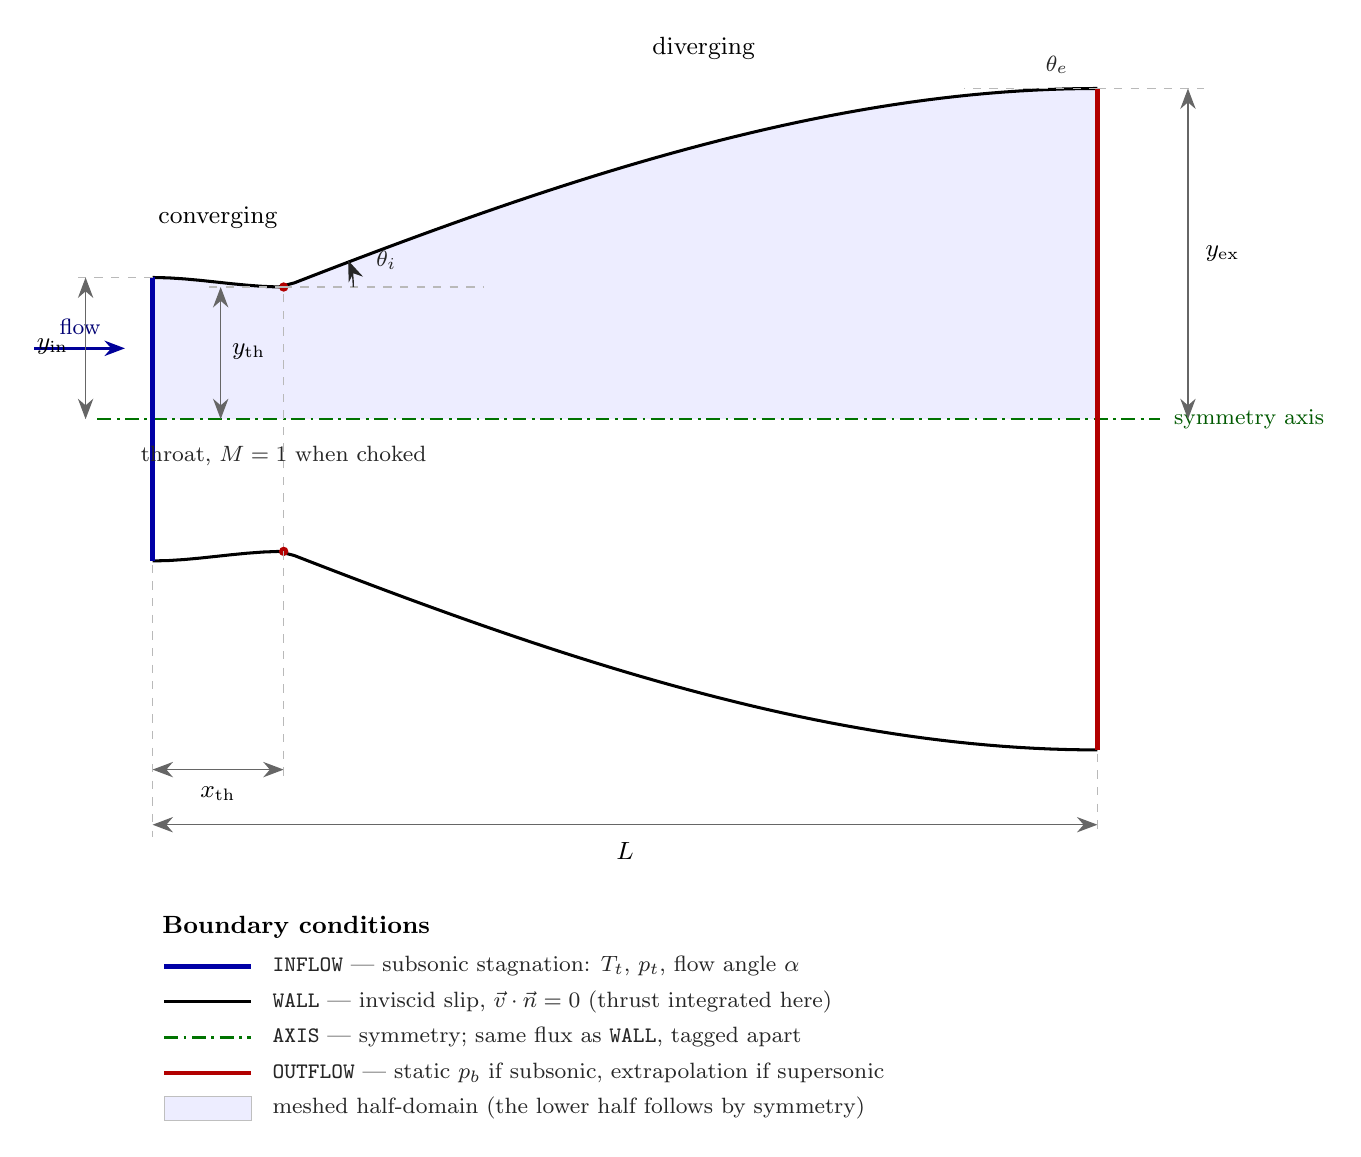
\begin{tikzpicture}[
  >={Stealth[length=2.6mm]},
  wall/.style   = {line width=1.1pt, black},
  axis/.style   = {line width=0.9pt, green!45!black, dash pattern=on 5pt off 2pt on 1pt off 2pt},
  inflow/.style = {line width=1.6pt, blue!65!black},
  outflow/.style= {line width=1.6pt, red!70!black},
  dim/.style    = {<->, gray!80!black, line width=0.5pt},
  guide/.style  = {gray!55, line width=0.4pt, dashed},
  lbl/.style    = {font=\small},
  slbl/.style   = {font=\footnotesize, gray!30!black},
]

%% ---- computational half-domain (shaded) --------------------------------
\fill[blue!7]
  plot coordinates {(0.0000,1.8000) (0.2000,1.7952) (0.4000,1.7824) (0.6000,1.7641) (0.8000,1.7429) (1.0000,1.7214) (1.2000,1.7019) (1.4000,1.6870) (1.6000,1.6793) (1.8000,1.7311) (2.0000,1.8087) (2.2000,1.8858) (2.4000,1.9625) (2.6000,2.0386) (2.8000,2.1141) (3.0000,2.1890) (3.2000,2.2633) (3.4000,2.3368) (3.6000,2.4095) (3.8000,2.4815) (4.0000,2.5526) (4.2000,2.6228) (4.4000,2.6921) (4.6000,2.7604) (4.8000,2.8277) (5.0000,2.8940) (5.2000,2.9591) (5.4000,3.0230) (5.6000,3.0858) (5.8000,3.1473) (6.0000,3.2076) (6.2000,3.2665) (6.4000,3.3240) (6.6000,3.3801) (6.8000,3.4348) (7.0000,3.4880) (7.2000,3.5396) (7.4000,3.5896) (7.6000,3.6380) (7.8000,3.6847) (8.0000,3.7297) (8.2000,3.7729) (8.4000,3.8143) (8.6000,3.8539) (8.8000,3.8915) (9.0000,3.9272) (9.2000,3.9610) (9.4000,3.9927) (9.6000,4.0223) (9.8000,4.0498) (10.0000,4.0751) (10.2000,4.0983) (10.4000,4.1192) (10.6000,4.1377) (10.8000,4.1540) (11.0000,4.1679) (11.2000,4.1793) (11.4000,4.1883) (11.6000,4.1948) (11.8000,4.1987) (12.0000,4.2000)} -- (12,0) -- (0,0) -- cycle;

%% ---- walls --------------------------------------------------------------
\draw[wall] plot coordinates {(0.0000,1.8000) (0.2000,1.7952) (0.4000,1.7824) (0.6000,1.7641) (0.8000,1.7429) (1.0000,1.7214) (1.2000,1.7019) (1.4000,1.6870) (1.6000,1.6793) (1.8000,1.7311) (2.0000,1.8087) (2.2000,1.8858) (2.4000,1.9625) (2.6000,2.0386) (2.8000,2.1141) (3.0000,2.1890) (3.2000,2.2633) (3.4000,2.3368) (3.6000,2.4095) (3.8000,2.4815) (4.0000,2.5526) (4.2000,2.6228) (4.4000,2.6921) (4.6000,2.7604) (4.8000,2.8277) (5.0000,2.8940) (5.2000,2.9591) (5.4000,3.0230) (5.6000,3.0858) (5.8000,3.1473) (6.0000,3.2076) (6.2000,3.2665) (6.4000,3.3240) (6.6000,3.3801) (6.8000,3.4348) (7.0000,3.4880) (7.2000,3.5396) (7.4000,3.5896) (7.6000,3.6380) (7.8000,3.6847) (8.0000,3.7297) (8.2000,3.7729) (8.4000,3.8143) (8.6000,3.8539) (8.8000,3.8915) (9.0000,3.9272) (9.2000,3.9610) (9.4000,3.9927) (9.6000,4.0223) (9.8000,4.0498) (10.0000,4.0751) (10.2000,4.0983) (10.4000,4.1192) (10.6000,4.1377) (10.8000,4.1540) (11.0000,4.1679) (11.2000,4.1793) (11.4000,4.1883) (11.6000,4.1948) (11.8000,4.1987) (12.0000,4.2000)};
\draw[wall] plot coordinates {(0.0000,-1.8000) (0.2000,-1.7952) (0.4000,-1.7824) (0.6000,-1.7641) (0.8000,-1.7429) (1.0000,-1.7214) (1.2000,-1.7019) (1.4000,-1.6870) (1.6000,-1.6793) (1.8000,-1.7311) (2.0000,-1.8087) (2.2000,-1.8858) (2.4000,-1.9625) (2.6000,-2.0386) (2.8000,-2.1141) (3.0000,-2.1890) (3.2000,-2.2633) (3.4000,-2.3368) (3.6000,-2.4095) (3.8000,-2.4815) (4.0000,-2.5526) (4.2000,-2.6228) (4.4000,-2.6921) (4.6000,-2.7604) (4.8000,-2.8277) (5.0000,-2.8940) (5.2000,-2.9591) (5.4000,-3.0230) (5.6000,-3.0858) (5.8000,-3.1473) (6.0000,-3.2076) (6.2000,-3.2665) (6.4000,-3.3240) (6.6000,-3.3801) (6.8000,-3.4348) (7.0000,-3.4880) (7.2000,-3.5396) (7.4000,-3.5896) (7.6000,-3.6380) (7.8000,-3.6847) (8.0000,-3.7297) (8.2000,-3.7729) (8.4000,-3.8143) (8.6000,-3.8539) (8.8000,-3.8915) (9.0000,-3.9272) (9.2000,-3.9610) (9.4000,-3.9927) (9.6000,-4.0223) (9.8000,-4.0498) (10.0000,-4.0751) (10.2000,-4.0983) (10.4000,-4.1192) (10.6000,-4.1377) (10.8000,-4.1540) (11.0000,-4.1679) (11.2000,-4.1793) (11.4000,-4.1883) (11.6000,-4.1948) (11.8000,-4.1987) (12.0000,-4.2000)};

%% ---- symmetry axis ------------------------------------------------------
\draw[axis] (-0.7,0) -- (12.8,0);
\node[slbl, green!35!black, anchor=west] at (12.85,0) {symmetry axis};

%% ---- inflow and outflow planes -----------------------------------------
\draw[inflow]  (0,0) -- (0,1.8000);
\draw[inflow]  (0,0) -- (0,-1.8000);
\draw[outflow] (12,0) -- (12,4.2000);
\draw[outflow] (12,0) -- (12,-4.2000);

%% ---- flow direction -----------------------------------------------------
\draw[->, blue!60!black, line width=0.9pt] (-1.5,0.9) -- (-0.35,0.9);
\node[slbl, blue!45!black, anchor=south] at (-0.92,0.95) {flow};

%% ---- throat -------------------------------------------------------------
\draw[guide] (1.6656,-1.6787) -- (1.6656,1.6787);
\fill[red!70!black] (1.6656,1.6787) circle (1.7pt);
\fill[red!70!black] (1.6656,-1.6787) circle (1.7pt);

%% ---- dimensions ---------------------------------------------------------
\draw[guide] (0,1.8000) -- (-1.05,1.8000);
\draw[dim]   (-0.85,0) -- (-0.85,1.8000);
\node[lbl, anchor=east] at (-0.95,0.92) {$y_{\mathrm{in}}$};

\draw[guide] (1.6656,1.6787) -- (0.6656,1.6787);
\draw[dim]   (0.8656,0) -- (0.8656,1.6787);
\node[lbl, anchor=west] at (0.8856,0.86) {$y_{\mathrm{th}}$};

\draw[guide] (12,4.2000) -- (13.35,4.2000);
\draw[dim]   (13.15,0) -- (13.15,4.2000);
\node[lbl, anchor=west] at (13.25,2.1) {$y_{\mathrm{ex}}$};

\draw[dim] (0,-5.15) -- (12,-5.15);
\node[lbl, anchor=north] at (6,-5.25) {$L$};
\draw[dim] (0,-4.45) -- (1.6656,-4.45);
\node[lbl, anchor=north] at (0.83,-4.55) {$x_{\mathrm{th}}$};
\draw[guide] (0,-1.85) -- (0,-5.3);
\draw[guide] (1.6656,-1.6787) -- (1.6656,-4.6);
\draw[guide] (12,-4.25) -- (12,-5.3);

%% ---- wall angles --------------------------------------------------------
\draw[guide] (1.6656,1.6787) -- (4.2,1.6787);
\draw[->, gray!30!black, line width=0.5pt] (2.55,1.6787) arc (0:22:0.9);
\node[slbl, anchor=west] at (2.72,2.02) {$\theta_i$};

\draw[guide] (12,4.2000) -- (10.3,4.2000);
\node[slbl, anchor=south east] at (11.75,4.26) {$\theta_e$};

%% ---- region labels ------------------------------------------------------
\node[lbl, anchor=south] at (0.83,2.30) {converging};
\node[lbl, anchor=south] at (7.0,4.45)  {diverging};
\node[slbl, anchor=north] at (1.6656,-0.22) {throat, $M = 1$ when choked};

%% ---- boundary-condition legend -----------------------------------------
\begin{scope}[shift={(0,-7.4)}]
  \node[lbl, anchor=west] at (0,0.95) {\textbf{Boundary conditions}};
  \draw[inflow]  (0.15,0.45) -- (1.25,0.45);
  \node[slbl, anchor=west] at (1.4,0.45)
    {\texttt{INFLOW} --- subsonic stagnation: $T_t$, $p_t$, flow angle $\alpha$};
  \draw[wall]    (0.15,0.00) -- (1.25,0.00);
  \node[slbl, anchor=west] at (1.4,0.00)
    {\texttt{WALL} --- inviscid slip, $\vec{v}\cdot\vec{n} = 0$ (thrust integrated here)};
  \draw[axis]    (0.15,-0.45) -- (1.25,-0.45);
  \node[slbl, anchor=west] at (1.4,-0.45)
    {\texttt{AXIS} --- symmetry; same flux as \texttt{WALL}, tagged apart};
  \draw[outflow] (0.15,-0.90) -- (1.25,-0.90);
  \node[slbl, anchor=west] at (1.4,-0.90)
    {\texttt{OUTFLOW} --- static $p_b$ if subsonic, extrapolation if supersonic};
  \fill[blue!7] (0.15,-1.50) rectangle (1.25,-1.20);
  \draw[gray!50, line width=0.3pt] (0.15,-1.50) rectangle (1.25,-1.20);
  \node[slbl, anchor=west] at (1.4,-1.35)
    {meshed half-domain (the lower half follows by symmetry)};
\end{scope}

\end{tikzpicture}

\end{document}
}
  \caption{Nozzle geometry, design variables and boundary conditions.  The
    shaded region is the half-domain that is actually meshed.  The wall shown is
    the \code{'bell'} contour at $\mathrm{AR} = 2.5019$, $x_{\mathrm{th}} = 0.1388$.}
  \label{fig:geometry}
\end{figure}

\subsection{Design variables}

The wall half-height $y_{\mathrm{wall}}(x; \avec)$ is controlled by
\begin{equation}
  \avec = \bigl(\mathrm{AR},\; x_{\mathrm{th}},\; y_{\mathrm{th}},\;
                y_{\mathrm{in}},\; L,\; \theta_i,\; \theta_e,\; w_1,\; w_2\bigr),
\end{equation}
listed in Table~\ref{tab:design}.  Every one of them is differentiable
(Section~\ref{sec:adjoint}).

\begin{table}[H]
  \centering
  \small
  \begin{tabular}{llp{8.4cm}}
    \toprule
    Symbol & Code name & Meaning \\
    \midrule
    $\mathrm{AR}$          & \code{area\_ratio}         & exit-to-throat area ratio, Eq.~\eqref{eq:arearatio} \\
    $x_{\mathrm{th}}$      & \code{throat\_x}           & throat location as a fraction of $L$ \\
    $y_{\mathrm{th}}$      & \code{throat\_half\_height}& throat half-height [m]; scales the nozzle \\
    $y_{\mathrm{in}}$      & \code{inlet\_half\_height} & inlet half-height [m]; must exceed $y_{\mathrm{th}}$ \\
    $L$                    & \code{length}              & axial length [m] \\
    $\theta_i$             & \code{theta\_initial\_deg} & wall angle just downstream of the throat \\
    $\theta_e$             & \code{theta\_exit\_deg}    & wall angle at the exit plane \\
    $w_1, w_2$             & \code{bezier\_w1/w2}       & B\'ezier shape weights \\
    \bottomrule
  \end{tabular}
  \caption{Design variables.}
  \label{tab:design}
\end{table}

\subsection{Converging section}

For $x \le x_{\mathrm{th}} L$, with $s = x/(x_{\mathrm{th}} L) \in [0,1]$, the wall is
a cubic Hermite with zero slope at both ends,
\begin{equation}
  y_{\mathrm{wall}}(s) = h_{00}(s)\, y_{\mathrm{in}} + h_{01}(s)\, y_{\mathrm{th}},
  \qquad
  \begin{aligned}
    h_{00}(s) &= 2s^{3} - 3s^{2} + 1, \\
    h_{01}(s) &= -2s^{3} + 3s^{2}.
  \end{aligned}
  \label{eq:converging}
\end{equation}
Because $y'(x_{\mathrm{th}}^{-}) = 0$, the point $x_{\mathrm{th}}$ really is a
stationary point of the wall, so ``throat'' and ``$x_{\mathrm{th}}$'' agree.

\subsection{Diverging section}

For $x > x_{\mathrm{th}} L$, with $s = (x - x_{\mathrm{th}}L)/(L - x_{\mathrm{th}}L)$
and $y_{\mathrm{ex}} = \mathrm{AR}\,y_{\mathrm{th}}$, five families are available.

\paragraph{\code{'conical'} --- straight wall.}
\begin{equation}
  y_{\mathrm{wall}} = y_{\mathrm{th}} + (y_{\mathrm{ex}} - y_{\mathrm{th}})\, s .
\end{equation}

\paragraph{\code{'bell'} and \code{'moc'} --- prescribed wall angles.}
A cubic Hermite with slopes $\tan\theta_i$ and $\tan\theta_e$ (converted to the
$s$ variable through $\mathrm{d}x/\mathrm{d}s$):
\begin{equation}
  y_{\mathrm{wall}} = h_{00} y_{\mathrm{th}} + h_{10} m_i
                    + h_{01} y_{\mathrm{ex}} + h_{11} m_e ,
  \qquad
  \begin{aligned}
    h_{10}(s) &= s^{3} - 2s^{2} + s, \\
    h_{11}(s) &= s^{3} - s^{2},
  \end{aligned}
  \label{eq:bell}
\end{equation}
with $m_i = \tan\theta_i \cdot \mathrm{d}x/\mathrm{d}s$ and similarly for $m_e$.
\code{'moc'} fixes $\theta_i = 30^{\circ}$, $\theta_e = 0$, the classical
Rao values.

\begin{quote}
\textbf{A slope discontinuity, on purpose.}  With $\theta_i > 0$ the wall slope
jumps from $0$ to $\tan\theta_i$ at the throat.  That sharp corner is the
idealisation used in minimum-length nozzle design --- it launches a centred
Prandtl--Meyer expansion fan --- and it is \emph{not} a defect.  It does,
however, put a singularity into the exact solution, which caps the achievable
order of accuracy.  Section~\ref{sec:verify} quantifies this.  Use
\code{'smooth'} or \code{'analytic'} for convergence studies.
\end{quote}

\paragraph{\code{'smooth'} --- $C^1$ throat.}
Equation~\eqref{eq:bell} with $\theta_i = 0$, so the wall slope is continuous
across the throat and the exact solution is smooth.

\paragraph{\code{'bezier'} --- two shape weights.}
A cubic B\'ezier in $s$ with interior control values
$c_k = y_{\mathrm{th}} + w_k (y_{\mathrm{ex}} - y_{\mathrm{th}})$:
\begin{equation}
  y_{\mathrm{wall}} = (1-s)^{3} y_{\mathrm{th}} + 3(1-s)^{2} s\, c_1
    + 3(1-s) s^{2} c_2 + s^{3} y_{\mathrm{ex}} .
  \label{eq:bezier}
\end{equation}
$(w_1, w_2) = (\tfrac13, \tfrac23)$ reproduces the conical wall; $w_1 = 0$ gives
a $C^1$ throat.  This is the most convenient family for gradient-based shape
optimisation, because $w_1$ and $w_2$ are bounded, dimensionless, and act
locally.

\paragraph{\code{'analytic'} --- the legacy verification contour.}
The fixed shape of the original MATLAB solver,
\begin{equation}
  t(x) = \pi \ln\!\bigl(1 + (e^{2}-1)\,x/L\bigr),
  \qquad
  y_{\mathrm{wall}} = 0.01\left(4 - \cos\tfrac{t}{2}\right)
                      \left(\cos t + 5 - \cos\tfrac{t}{2}\right),
  \label{eq:analytic}
\end{equation}
which runs from $y = 0.15$ at the inlet through a throat of $0.13989434$ at
$x = 0.138805$ to $y = 0.35$ at the exit, an area ratio of $2.50189$.  It ignores
\code{area\_ratio} and \code{throat\_x}; it exists so that results can be checked
against the original code.

%% =========================================================================
\section{Discretisation}

\subsection{Mesh}

\begin{figure}[H]
  \centering
  \resizebox{0.95\textwidth}{!}{%% ==========================================================================
%%  dgnozzle -- logical grid to physical nozzle mapping
%% ==========================================================================
\ifdefined\DGNOZZLEEMBEDDED\else
\documentclass[tikz,border=6pt]{standalone}
\usepackage{amsmath}
\usetikzlibrary{arrows.meta,calc}
\begin{document}
\fi

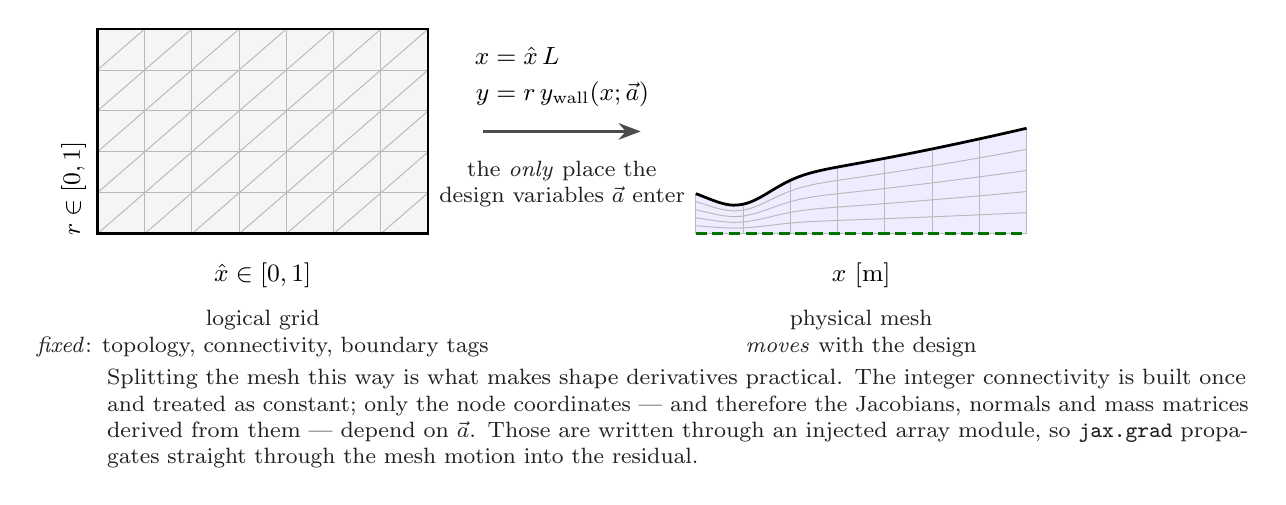
\begin{tikzpicture}[
  >={Stealth[length=2.8mm]},
  grid/.style = {gray!55, line width=0.35pt},
  bd/.style   = {line width=1.0pt},
  lbl/.style  = {font=\small},
  slbl/.style = {font=\footnotesize, gray!25!black},
]

%% ---- logical square ------------------------------------------------------
\begin{scope}
  \fill[black!4] (0,0) rectangle (4.2,2.6);
  \foreach \i in {0,...,7} \draw[grid] (\i*0.6,0) -- (\i*0.6,2.6);
  \foreach \j in {0,...,5} \draw[grid] (0,\j*0.52) -- (4.2,\j*0.52);
  \foreach \i in {0,...,6} \foreach \j in {0,...,4}
    \draw[grid] (\i*0.6,\j*0.52) -- (\i*0.6+0.6,\j*0.52+0.52);
  \draw[bd] (0,0) rectangle (4.2,2.6);
  \node[lbl, anchor=north] at (2.1,-0.25) {$\hat{x} \in [0,1]$};
  \node[lbl, anchor=east, rotate=90] at (-0.3,1.3) {$r \in [0,1]$};
  \node[slbl, anchor=north, align=center] at (2.1,-0.85)
    {logical grid\\ \emph{fixed}: topology, connectivity, boundary tags};
\end{scope}

%% ---- the map -------------------------------------------------------------
\draw[->, line width=1.2pt, black!70] (4.9,1.3) -- (6.9,1.3);
\node[lbl, anchor=south, align=center] at (5.9,1.45)
  {$\displaystyle \begin{aligned} x &= \hat{x}\,L\\[-1pt]
    y &= r\, y_{\mathrm{wall}}(x;\vec{a})\end{aligned}$};
\node[slbl, anchor=north, align=center, text width=3.4cm] at (5.9,1.05)
  {the \emph{only} place the design variables $\vec{a}$ enter};

%% ---- physical nozzle -----------------------------------------------------
\begin{scope}[xshift=7.6cm]
  \def\wall#1{0.62 + 1.05*(#1)*(#1) - 0.22*(#1)}
  \fill[blue!7] plot[domain=0:4.2,samples=60]
        (\x, {0.62 - 0.30*exp(-((\x-0.55)/0.55)^2) + 0.30*(\x/4.2)^1.35*2.4})
        -- (4.2,0) -- (0,0) -- cycle;
  \foreach \j in {0,...,5}
    \draw[grid] plot[domain=0:4.2,samples=60]
      (\x, {(\j/5)*(0.62 - 0.30*exp(-((\x-0.55)/0.55)^2) + 0.30*(\x/4.2)^1.35*2.4)});
  \foreach \i in {0,...,7}
    \draw[grid] (\i*0.6,0) --
      (\i*0.6, {0.62 - 0.30*exp(-((\i*0.6-0.55)/0.55)^2) + 0.30*(\i*0.6/4.2)^1.35*2.4});
  \draw[bd] plot[domain=0:4.2,samples=80]
      (\x, {0.62 - 0.30*exp(-((\x-0.55)/0.55)^2) + 0.30*(\x/4.2)^1.35*2.4});
  \draw[bd, green!45!black, dash pattern=on 4pt off 2pt] (0,0) -- (4.2,0);
  \node[lbl, anchor=north] at (2.1,-0.25) {$x$ [m]};
  \node[slbl, anchor=north, align=center] at (2.1,-0.85)
    {physical mesh\\ \emph{moves} with the design};
\end{scope}

\node[slbl, align=left, anchor=north west, text width=14.5cm] at (0,-1.6)
  {Splitting the mesh this way is what makes shape derivatives practical.  The
   integer connectivity is built once and treated as constant; only the node
   coordinates --- and therefore the Jacobians, normals and mass matrices
   derived from them --- depend on $\vec{a}$.  Those are written through an
   injected array module, so \texttt{jax.grad} propagates straight through the
   mesh motion into the residual.};

\end{tikzpicture}

\ifdefined\DGNOZZLEEMBEDDED\else
\end{document}
\fi
}
  \caption{The mesh is built as a fixed logical grid plus a design-dependent
    map.  Only the map depends on $\avec$, which is what makes shape derivatives
    tractable.}
  \label{fig:meshmap}
\end{figure}

A structured $n_x \times n_r$ grid of cells is laid out in logical coordinates
$(\hat{x}, r) \in [0,1]^2$ and mapped to the nozzle by
\begin{equation}
  x = \hat{x} L, \qquad y = r\, y_{\mathrm{wall}}(x; \avec).
  \label{eq:meshmap}
\end{equation}
Each cell becomes one quadrilateral or two triangles.  Refinement level
$\mathrm{ref}$ subdivides each cell $2^{\mathrm{ref}}$ ways per direction, so the
element count is $n_x n_r 4^{\mathrm{ref}}$ (doubled for triangles).

Axial nodes may be clustered toward the throat, where the solution varies
fastest.  The base distribution is generated from a target spacing
\begin{equation}
  h(\hat{x}) = 1 + (\sigma - 1)
    \left(1 - e^{-\left((\hat{x} - x_{\mathrm{th}})/w\right)^{2}}\right),
\end{equation}
integrated and inverted, with $\sigma$ the far-field-to-throat spacing ratio.
Refinement then subdivides that base distribution linearly, so the node set at
one refinement level is a subset of the next.

\subsection{Reference elements}

\begin{figure}[H]
  \centering
  \resizebox{\textwidth}{!}{%% ==========================================================================
%%  dgnozzle -- reference elements, node ordering and edge numbering
%% ==========================================================================
\documentclass[tikz,border=6pt]{standalone}
\usepackage{amsmath}
\usetikzlibrary{arrows.meta,calc,positioning}
\begin{document}

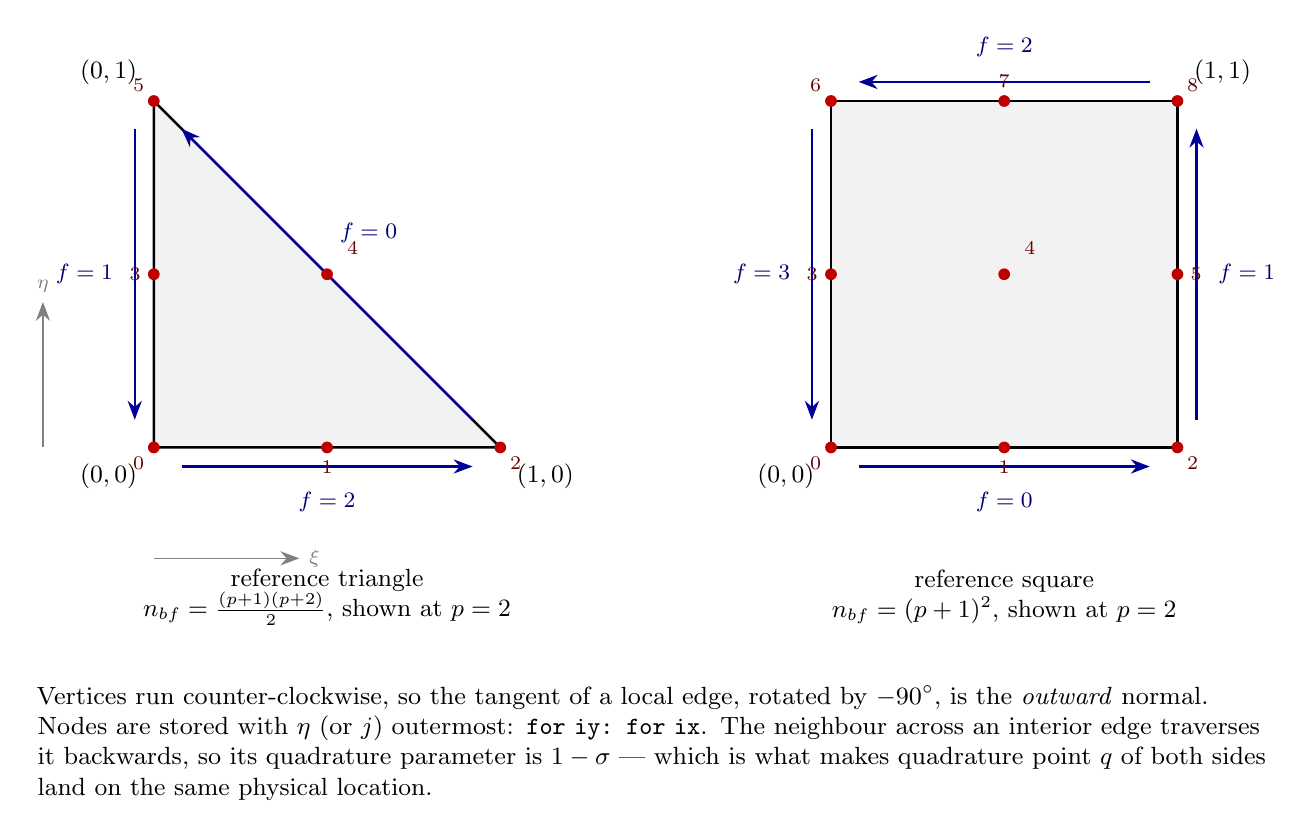
\begin{tikzpicture}[
  >={Stealth[length=2.4mm]},
  node distance=0pt,
  edgearr/.style = {->, blue!60!black, line width=0.8pt},
  nd/.style      = {circle, fill=red!75!black, inner sep=1.5pt},
  ndlbl/.style   = {font=\scriptsize, red!40!black},
  elbl/.style    = {font=\footnotesize, blue!45!black},
  vlbl/.style    = {font=\small},
  capt/.style    = {font=\small},
]

%% ------------------------------------------------------------------ TRIANGLE
\begin{scope}[scale=4.4]
  \fill[black!5] (0,0) -- (1,0) -- (0,1) -- cycle;
  \draw[line width=0.9pt] (0,0) -- (1,0) -- (0,1) -- cycle;

  % local edges: edge f is opposite vertex f, traversed CCW
  \draw[edgearr] (0.92,0.08) -- (0.08,0.92);      % f = 0 : v1 -> v2
  \draw[edgearr] (-0.055,0.92) -- (-0.055,0.08);  % f = 1 : v2 -> v0
  \draw[edgearr] (0.08,-0.055) -- (0.92,-0.055);  % f = 2 : v0 -> v1
  \node[elbl] at (0.62,0.62) {$f=0$};
  \node[elbl, anchor=east] at (-0.09,0.5) {$f=1$};
  \node[elbl, anchor=north] at (0.5,-0.10) {$f=2$};

  % p = 2 Lagrange nodes, in storage order
  \foreach \p/\i in {{0,0}/0, {0.5,0}/1, {1,0}/2, {0,0.5}/3, {0.5,0.5}/4, {0,1}/5}
    { \node[nd] at (\p) {}; }
  \node[ndlbl, anchor=north east] at (0,0)      {$0$};
  \node[ndlbl, anchor=north]      at (0.5,-0.01){$1$};
  \node[ndlbl, anchor=north west] at (1,0)      {$2$};
  \node[ndlbl, anchor=east]       at (-0.01,0.5){$3$};
  \node[ndlbl, anchor=south west] at (0.53,0.53){$4$};
  \node[ndlbl, anchor=south east] at (0,1)      {$5$};

  \node[vlbl, anchor=north east] at (-0.02,-0.02) {$(0,0)$};
  \node[vlbl, anchor=north west] at (1.02,-0.02)  {$(1,0)$};
  \node[vlbl, anchor=south east] at (-0.02,1.02)  {$(0,1)$};

  \draw[->, gray, line width=0.5pt] (0,-0.32) -- (0.42,-0.32)
        node[right, font=\scriptsize, gray] {$\xi$};
  \draw[->, gray, line width=0.5pt] (-0.32,0) -- (-0.32,0.42)
        node[above, font=\scriptsize, gray] {$\eta$};
\end{scope}

\node[capt, align=center] at (2.2,-1.9)
  {reference triangle\\ $n_{bf} = \tfrac{(p+1)(p+2)}{2}$, shown at $p=2$};

%% ------------------------------------------------------------------ QUAD
\begin{scope}[xshift=8.6cm, scale=4.4]
  \fill[black!5] (0,0) rectangle (1,1);
  \draw[line width=0.9pt] (0,0) rectangle (1,1);

  \draw[edgearr] (0.08,-0.055) -- (0.92,-0.055);   % f = 0
  \draw[edgearr] (1.055,0.08) -- (1.055,0.92);     % f = 1
  \draw[edgearr] (0.92,1.055) -- (0.08,1.055);     % f = 2
  \draw[edgearr] (-0.055,0.92) -- (-0.055,0.08);   % f = 3
  \node[elbl, anchor=north] at (0.5,-0.10) {$f=0$};
  \node[elbl, anchor=west]  at (1.09,0.5)  {$f=1$};
  \node[elbl, anchor=south] at (0.5,1.10)  {$f=2$};
  \node[elbl, anchor=east]  at (-0.09,0.5) {$f=3$};

  \foreach \x in {0,0.5,1}
    \foreach \y in {0,0.5,1}
      { \node[nd] at (\x,\y) {}; }
  \node[ndlbl, anchor=north east] at (0,0)       {$0$};
  \node[ndlbl, anchor=north]      at (0.5,-0.01) {$1$};
  \node[ndlbl, anchor=north west] at (1,0)       {$2$};
  \node[ndlbl, anchor=east]       at (-0.01,0.5) {$3$};
  \node[ndlbl, anchor=south west] at (0.53,0.53) {$4$};
  \node[ndlbl, anchor=west]       at (1.01,0.5)  {$5$};
  \node[ndlbl, anchor=south east] at (0,1)       {$6$};
  \node[ndlbl, anchor=south]      at (0.5,1.01)  {$7$};
  \node[ndlbl, anchor=south west] at (1,1)       {$8$};

  \node[vlbl, anchor=north east] at (-0.02,-0.02) {$(0,0)$};
  \node[vlbl, anchor=south west] at (1.02,1.02)   {$(1,1)$};
\end{scope}

\node[capt, align=center] at (10.8,-1.9)
  {reference square\\ $n_{bf} = (p+1)^2$, shown at $p=2$};

\node[capt, align=left, anchor=north west, text width=15.6cm] at (-1.6,-2.9)
  {Vertices run counter-clockwise, so the tangent of a local edge, rotated by
   $-90^\circ$, is the \emph{outward} normal.  Nodes are stored with
   $\eta$ (or $j$) outermost: \texttt{for iy: for ix}.  The neighbour across an
   interior edge traverses it backwards, so its quadrature parameter is
   $1-\sigma$ --- which is what makes quadrature point $q$ of both sides land on
   the same physical location.};

\end{tikzpicture}

\end{document}
}
  \caption{Reference elements, Lagrange node ordering and local edge numbering.}
  \label{fig:refelem}
\end{figure}

The solution is expanded in a nodal Lagrange basis of order $p$ on each element,
\begin{equation}
  \Uvec_h(\xvec)\big|_{\Omega_e}
  = \sum_{i=1}^{n_{bf}} \Uvec_{e,i}\, \phi_i(\xi, \eta),
  \qquad
  n_{bf} =
  \begin{cases}
    \tfrac{1}{2}(p+1)(p+2) & \text{triangle},\\[2pt]
    (p+1)^{2}              & \text{quadrilateral}.
  \end{cases}
\end{equation}
The element geometry uses an independent Lagrange basis of order $Q$, so $Q = 1$
gives straight-sided elements and $Q = 2$ a quadratic (curved) wall.

The mapping from reference to physical coordinates and its Jacobian are
\begin{equation}
  \xvec(\xi,\eta) = \sum_{n} \xvec_n\, \psi_n(\xi,\eta),
  \qquad
  J = \frac{\partial(x,y)}{\partial(\xi,\eta)},
  \qquad
  \nabla_{\xvec}\phi_i = J^{-T}\nabla_{(\xi,\eta)}\phi_i .
\end{equation}

\subsection{Weak form}

Multiplying Eq.~\eqref{eq:euler} by a test function $\phi_i$, integrating over an
element and applying the divergence theorem gives the discrete statement
\begin{equation}
  \boxed{\;
  \int_{\Omega_e} \phi_i \frac{\partial \Uvec_h}{\partial t}\,\mathrm{d}\Omega
  =
  \int_{\Omega_e} \nabla \phi_i \cdot \vect{\mathcal{F}}(\Uvec_h)\,\mathrm{d}\Omega
  - \oint_{\partial \Omega_e} \phi_i\,
    \hat{F}\bigl(\Uvec_h^{+}, \Uvec_h^{-}, \nvec\bigr)\,\mathrm{d}s \;}
  \label{eq:weak}
\end{equation}
for every basis function $i$ and every element $e$.  Writing the right-hand side
as $-\vect{R}_e$ leaves the semi-discrete system
\begin{equation}
  M_e\, \dot{\Uvec}_e = -\vect{R}_e(\Uvec),
  \qquad
  (M_e)_{ij} = \int_{\Omega_e} \phi_i \phi_j\,\mathrm{d}\Omega .
  \label{eq:semidiscrete}
\end{equation}
The mass matrix is block diagonal --- an element couples to itself only --- so
$M^{-1}$ is applied as $n_{elem}$ independent $n_{bf} \times n_{bf}$ solves.

\begin{figure}[H]
  \centering
  \resizebox{0.95\textwidth}{!}{%% ==========================================================================
%%  dgnozzle -- how two elements couple: traces, normal, numerical flux
%% ==========================================================================
\documentclass[tikz,border=6pt]{standalone}
\usepackage{amsmath}
\usetikzlibrary{arrows.meta,calc,decorations.markings}
\begin{document}

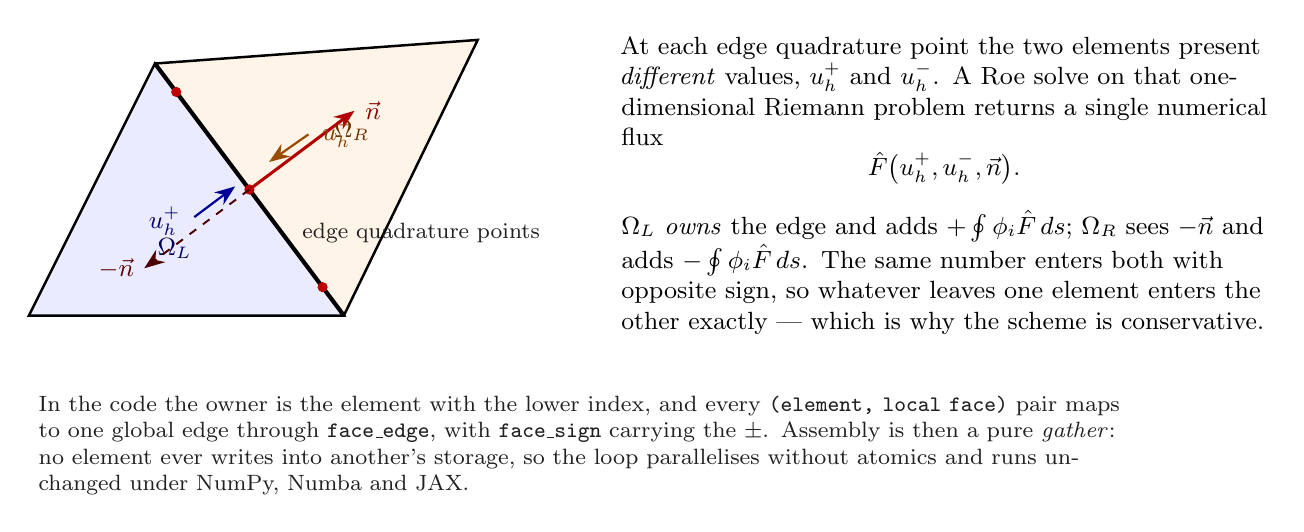
\begin{tikzpicture}[
  >={Stealth[length=2.6mm]},
  el/.style   = {line width=0.9pt},
  qp/.style   = {circle, fill=red!75!black, inner sep=1.3pt},
  lbl/.style  = {font=\small},
  slbl/.style = {font=\footnotesize, gray!25!black},
]

%% two triangles sharing an edge
\fill[blue!8]   (0,0) -- (4,0) -- (1.6,3.2) -- cycle;
\fill[orange!9] (4,0) -- (1.6,3.2) -- (5.7,3.5) -- cycle;
\draw[el] (0,0) -- (4,0) -- (1.6,3.2) -- cycle;
\draw[el] (4,0) -- (5.7,3.5) -- (1.6,3.2);

\draw[line width=1.5pt, black] (4,0) -- (1.6,3.2);

\node[lbl, blue!35!black]   at (1.85,0.85) {$\Omega_L$};
\node[lbl, orange!40!black] at (4.1,2.35)  {$\Omega_R$};

%% quadrature points on the shared edge
\foreach \t in {0.1127,0.5,0.8873}
  { \node[qp] at ($(4,0)!\t!(1.6,3.2)$) {}; }
\node[slbl, anchor=west] at (3.35,1.05) {edge quadrature points};

%% outward normal of the owner (L)
\coordinate (mid) at ($(4,0)!0.5!(1.6,3.2)$);
\draw[->, red!70!black, line width=1.1pt] (mid) -- ++(1.335,1.0)
      node[right, lbl, red!55!black] {$\vec{n}$};
\draw[->, red!30!black, line width=0.7pt, dashed] (mid) -- ++(-1.335,-1.0)
      node[left, lbl, red!35!black] {$-\vec{n}$};

%% traces
\draw[->, blue!60!black, line width=0.8pt] (2.1,1.25) -- (2.62,1.64);
\node[lbl, blue!45!black, anchor=east] at (2.05,1.2) {$u_h^{+}$};
\draw[->, orange!60!black, line width=0.8pt] (3.55,2.3) -- (3.05,1.95);
\node[lbl, orange!50!black, anchor=west] at (3.6,2.32) {$u_h^{-}$};

%% the Riemann problem
\node[lbl, align=left, anchor=west, text width=8.2cm] at (7.4,2.6)
  {At each edge quadrature point the two elements present
   \emph{different} values, $u_h^{+}$ and $u_h^{-}$.  A Roe solve on that
   one-dimensional Riemann problem returns a single numerical flux
   \[ \hat{F}\bigl(u_h^{+}, u_h^{-}, \vec{n}\bigr). \]};

\node[lbl, align=left, anchor=west, text width=8.2cm] at (7.4,0.55)
  {$\Omega_L$ \emph{owns} the edge and adds $+\oint \phi_i \hat{F}\,ds$;
   $\Omega_R$ sees $-\vec{n}$ and adds $-\oint \phi_i \hat{F}\,ds$.  The same
   number enters both with opposite sign, so whatever leaves one element
   enters the other exactly --- which is why the scheme is conservative.};

\node[slbl, align=left, anchor=north west, text width=13.8cm] at (0,-0.9)
  {In the code the owner is the element with the lower index, and every
   \texttt{(element, local face)} pair maps to one global edge through
   \texttt{face\_edge}, with \texttt{face\_sign} carrying the $\pm$.  Assembly is
   then a pure \emph{gather}: no element ever writes into another's storage, so
   the loop parallelises without atomics and runs unchanged under NumPy, Numba
   and JAX.};

\end{tikzpicture}

\end{document}
}
  \caption{Elements communicate only through the numerical flux on their shared
    edge.  The same value enters both with opposite sign, which is what makes
    the scheme conservative.}
  \label{fig:coupling}
\end{figure}

\subsection{Quadrature}

Volume integrals use symmetric positive-weight rules on the triangle (a
Duffy-collapsed Gauss--Jacobi rule for degree $\ge 3$) and tensor-product
Gauss--Legendre on the quadrilateral; edge integrals use Gauss--Legendre on
$[0,1]$.  The degrees are
\begin{equation}
  d_{\mathrm{vol}} = 2p + 1 + 2(Q-1),
  \qquad
  d_{\mathrm{edge}} = 2p + Q .
\end{equation}

\begin{quote}
\textbf{Positive weights are not optional.}  The Dunavant degree-3 rule used by
the original code has a negative first weight, $-0.28125$.  A negative weight can
destroy the positive definiteness of $M_e$ and lets the entropy-error integral
--- a sum of squares --- go negative.  Every rule here has strictly positive
weights, checked against exact monomial integrals in the test suite.
\end{quote}

%% =========================================================================
\section{Numerical flux}

The interface flux is Roe's approximate Riemann solver,
\begin{equation}
  \hat{F}(\Uvec^{+}, \Uvec^{-}, \nvec)
  = \tfrac{1}{2}\left(\Fvec(\Uvec^{+})\!\cdot\!\nvec
                    + \Fvec(\Uvec^{-})\!\cdot\!\nvec\right)
  - \tfrac{1}{2}\left|\hat{A}\right| \left(\Uvec^{-} - \Uvec^{+}\right),
  \label{eq:roe}
\end{equation}
where $\hat{A}$ is the flux Jacobian evaluated at the Roe-averaged state
\begin{equation}
  \hat{u} = \frac{\sqrt{\rho^{+}}\,u^{+} + \sqrt{\rho^{-}}\,u^{-}}
                 {\sqrt{\rho^{+}} + \sqrt{\rho^{-}}},
  \quad \text{(and likewise for } \hat{v},\ \hat{H}\text{)},
  \qquad
  \hat{a}^{2} = (\gamma - 1)\left(\hat{H} - \tfrac{1}{2}\hat{q}^{2}\right).
\end{equation}
The dissipation term is evaluated in factored form rather than by assembling
$|\hat{A}|$: with
$\Delta(\cdot) = (\cdot)^{-} - (\cdot)^{+}$,
\begin{align}
  G_1 &= (\gamma-1)\left(\tfrac{1}{2}\hat{q}^{2}\Delta\rho
         - \hat{u}\,\Delta(\rho u) - \hat{v}\,\Delta(\rho v) + \Delta(\rho E)\right),\\
  G_2 &= -\hat{u}_n \Delta\rho + \Delta(\rho u)\, n_x + \Delta(\rho v)\, n_y,\\
  s_1 &= \tfrac{1}{2}\left(|\lambda_1| + |\lambda_2|\right), \qquad
  s_2 = \tfrac{1}{2}\left(|\lambda_1| - |\lambda_2|\right),\\
  C_1 &= \frac{G_1}{\hat{a}^{2}}\left(s_1 - |\lambda_3|\right) + \frac{G_2}{\hat{a}} s_2,
  \qquad
  C_2 = \frac{G_1}{\hat{a}} s_2 + \left(s_1 - |\lambda_3|\right) G_2 .
\end{align}

\paragraph{Entropy fix.}
An unmodified Roe flux admits a non-physical expansion shock where an eigenvalue
passes through zero --- which happens at the throat of every choked nozzle.  The
Harten--Hyman fix replaces small eigenvalues by a smooth quadratic,
\begin{equation}
  |\lambda| \leftarrow
  \begin{cases}
    \dfrac{\lambda^{2} + \epsilon^{2}}{2\epsilon}, & |\lambda| < \epsilon,\\[8pt]
    |\lambda|, & \text{otherwise},
  \end{cases}
  \qquad \epsilon = 0.05\,\hat{a}.
  \label{eq:entropyfix}
\end{equation}

%% =========================================================================
\section{Boundary conditions}
\label{sec:bc}

The number of conditions that may be imposed equals the number of \emph{incoming}
characteristics, read off the eigenvalues in Eq.~\eqref{eq:eigs} with $\nvec$
the outward normal.

\subsection{Inviscid wall and symmetry axis}

Both are impermeable: $\vect{v}\cdot\nvec = 0$.  Removing the normal velocity and
recovering the pressure from the remaining energy gives a flux that transmits
pressure but no mass or energy,
\begin{equation}
  p_b = (\gamma - 1)\left(\rho E - \tfrac{1}{2}\rho\,|\vect{v}_{\parallel}|^{2}\right),
  \qquad
  \hat{F} = \bigl(0,\; p_b n_x,\; p_b n_y,\; 0\bigr)^{T}.
  \label{eq:wall}
\end{equation}
The contoured wall and the symmetry axis use the same flux but carry different
tags, so that thrust can be integrated over the wall alone.

\subsection{Subsonic stagnation inflow}

Three characteristics enter, one leaves.  The outgoing one carries the interior
Riemann invariant
\begin{equation}
  J^{+} = u_n + \frac{2a}{\gamma - 1}.
\end{equation}
Combining it with the isentropic stagnation relations and a prescribed flow
direction $\hat{d} = (\cos\alpha, \sin\alpha)$ gives a quadratic for the inflow
Mach number,
\begin{equation}
  \underbrace{\left(\tfrac{\gamma-1}{2}\beta - n_d^{2}\right)}_{\textstyle A} M^{2}
  \underbrace{-\,\tfrac{4 n_d}{\gamma-1}}_{\textstyle B} M
  + \underbrace{\left(\beta - \left(\tfrac{2}{\gamma-1}\right)^{2}\right)}_{\textstyle C}
  = 0,
  \qquad
  \beta = \left(\frac{J^{+}}{a_t}\right)^{2},\quad n_d = \nvec\cdot\hat{d}.
  \label{eq:inflowquad}
\end{equation}
The \emph{smallest non-negative} root is the physical branch; the boundary state
then follows from the isentropic relations and total enthalpy
$H_b = a_t^{2}/(\gamma-1)$.

\begin{quote}
\textbf{Root selection.}  The legacy implementation always took
$(-B + \sqrt{B^{2}-4AC})/2A$.  That is the physical root only while $A > 0$; when
the leading coefficient changes sign --- which happens for weak inflow --- it
returns a negative Mach number and the boundary state becomes meaningless.
\end{quote}

\subsection{Outflow}

If $u_n/a \ge 1$ the outflow is supersonic: no characteristic enters, nothing may
be imposed, and the interior state is extrapolated.  If it is subsonic, exactly
one condition is admissible.  Static pressure is set to $p_b$, while entropy and
the outgoing invariant are carried from the interior and the tangential velocity
is unchanged:
\begin{equation}
  \rho_b = \rho^{+}\left(\frac{p_b}{p^{+}}\right)^{1/\gamma},
  \qquad
  u_{n,b} = u_n^{+} + \frac{2}{\gamma-1}\left(a^{+} - a_b\right),
  \qquad
  \vect{v}_{t,b} = \vect{v}_t^{+} .
  \label{eq:outflow}
\end{equation}
The two branches are selected by the local normal Mach number, so a shock
crossing the exit plane during the transient is handled without special cases.

\begin{quote}
\textbf{The legacy solver had no back pressure.}  Its outflow condition always
extrapolated, so the \code{p\_back\_ratio} input never reached the flow.  Every
operating point with a shock in the nozzle --- that is, most of the interesting
ones --- was therefore unreachable.
\end{quote}

%% =========================================================================
\section{Time integration}

Equation~\eqref{eq:semidiscrete} is marched in pseudo-time to steady state with
an element-local step,
\begin{equation}
  \Delta t_e
  = \frac{\mathrm{CFL}}{2p+1}\,
    \frac{2 A_e}{\displaystyle\sum_{f \in \partial\Omega_e} s_f\, \ell_f},
  \label{eq:dt}
\end{equation}
where $A_e$ is the element area, $\ell_f$ the length of face $f$ and $s_f$ the
maximum signal speed there.  The $1/(2p+1)$ factor is the standard
order-dependent restriction for explicit DG.

Two schemes are available.  \code{'rk4'} is the classical four-stage method, with
the local step frozen at the first stage (the intermediate stages are not meant
to be time-accurate).  \code{'ssprk3'} is the three-stage strong-stability-preserving
method,
\begin{equation}
  \begin{aligned}
    \Uvec^{(1)} &= \Uvec^{n} + \Delta t\, \mathcal{L}(\Uvec^{n}),\\
    \Uvec^{(2)} &= \tfrac{3}{4}\Uvec^{n} + \tfrac{1}{4}
      \left(\Uvec^{(1)} + \Delta t\, \mathcal{L}(\Uvec^{(1)})\right),\\
    \Uvec^{n+1} &= \tfrac{1}{3}\Uvec^{n} + \tfrac{2}{3}
      \left(\Uvec^{(2)} + \Delta t\, \mathcal{L}(\Uvec^{(2)})\right),
  \end{aligned}
  \qquad \mathcal{L} = -M^{-1}\vect{R}.
\end{equation}
Each SSP stage is a convex combination of forward-Euler updates, which is exactly
the structure the positivity limiter assumes --- so \code{'ssprk3'} plus
\code{'positivity'} carries a genuine positivity guarantee that \code{'rk4'} does
not.

\paragraph{Convergence measure.}  The march stops when
\begin{equation}
  \frac{\left\|\dot{\Uvec}\right\|_{\mathrm{rms}}}{\rho_t a_t / L}
  < \code{tolerance},
  \qquad
  \left\|\dot{\Uvec}\right\|_{\mathrm{rms}}
  = \sqrt{\frac{1}{4N}\sum \left(M^{-1}\vect{R}\right)^{2}} .
\end{equation}
The choice of denominator matters more than it looks.  Testing the
\emph{unnormalised} residual against a fixed threshold --- what the legacy solver
did --- makes ``converged'' mean different things on different meshes and at
different operating points.  But testing it \emph{relative to the first
iteration} is no better: it demands a tighter absolute residual the better the
initial guess is, so improving the initial condition makes the solver appear
slower and two runs started differently cannot be compared at all.  A fixed
physical scale, $\rho_t a_t / L$, is independent of both the mesh and the
starting field.  The legacy solver additionally tested the \emph{fourth}
Runge--Kutta stage's rate, which is not the residual at any state it holds.

%% =========================================================================
\section{Limiting}

At $p = 0$ the solution is constant per element and cannot oscillate.  At
$p \ge 1$ it can, and near a shock it does: the polynomial overshoots, pressure
or density goes negative at a quadrature point, and the Roe flux fails.

Both limiters act by shrinking the deviation from the cell average,
\begin{equation}
  \Uvec_{e,i}^{\mathrm{lim}} = \bar{\Uvec}_e
    + \theta_e \left(\Uvec_{e,i} - \bar{\Uvec}_e\right),
  \qquad \theta_e \in [0,1],
  \label{eq:limiter}
\end{equation}
which leaves the cell average untouched and is therefore \emph{conservative}.

\paragraph{Positivity (Zhang--Shu).}
$\theta_e$ is the largest value keeping $\rho$ and $p$ above small floors at
every point the scheme evaluates --- the volume quadrature points and the
element's own face quadrature points.  The density constraint is linear in
$\theta$ and solved in closed form; the pressure constraint is quadratic and
bracketed by bisection.  On a smooth solution $\theta_e = 1$ everywhere and the
limiter is exactly inactive, so full accuracy is retained.

\paragraph{Barth--Jespersen.}
Additionally bounds the solution by the neighbouring cell averages, damping the
oscillations themselves rather than only their consequences, at the cost of
clipping genuine extrema.

\paragraph{When a limiter cannot help.}
If the \emph{cell average} itself becomes non-physical, no scaling can repair it
--- at $\theta = 0$ the solution \emph{is} that average.  The code then floors
the average minimally, counts the repair, and reports it; a run needing repairs
should be rerun with a smaller \code{cfl}.  Separately, a limiter that switches
on and off between iterations parks the residual at a fixed level instead of
converging.  The solver detects that limit cycle, stops, and says so.

%% =========================================================================
\section{Quasi-one-dimensional reference solution}
\label{sec:quasi1d}

Quasi-1D theory serves two purposes: it is an exact reference to compare against,
and it is the initial condition.  As a starting field it saves a modest number
of iterations (about 15\% at $p = 0$, 3\% at $p = 1$ on the reference case); its
real value is robustness, since at $p = 2$ without $p$-continuation a uniform
start diverges where the quasi-1D start converges.

The area--Mach relation is
\begin{equation}
  \frac{A}{A^{*}} = \frac{1}{M}
  \left[\frac{2}{\gamma+1}\left(1 + \frac{\gamma-1}{2}M^{2}\right)
  \right]^{\frac{\gamma+1}{2(\gamma-1)}},
  \label{eq:areamach}
\end{equation}
monotone on each of the subsonic and supersonic branches and therefore invertible
by bracketed bisection.  The isentropic relations give
\begin{equation}
  \frac{p}{p_t} = \left(1 + \tfrac{\gamma-1}{2}M^{2}\right)^{-\frac{\gamma}{\gamma-1}},
  \qquad
  \frac{\rho}{\rho_t} = \left(1 + \tfrac{\gamma-1}{2}M^{2}\right)^{-\frac{1}{\gamma-1}},
  \qquad
  \frac{T}{T_t} = \left(1 + \tfrac{\gamma-1}{2}M^{2}\right)^{-1}.
\end{equation}

Across a normal shock,
\begin{equation}
  M_2^{2} = \frac{1 + \frac{\gamma-1}{2}M_1^{2}}{\gamma M_1^{2} - \frac{\gamma-1}{2}},
  \qquad
  \frac{p_2}{p_1} = \frac{2\gamma M_1^{2} - (\gamma-1)}{\gamma+1},
  \qquad
  \frac{A_2^{*}}{A_1^{*}} = \frac{p_{t1}}{p_{t2}} .
  \label{eq:shock}
\end{equation}

\subsection{Operating regimes}

Three critical back-pressure ratios divide the operating map:

\begin{table}[H]
  \centering
  \small
  \begin{tabular}{llp{7.6cm}}
    \toprule
    Ratio & Condition & Regime below it \\
    \midrule
    $(p_b/p_t)_1$ & $M = 1$ at the throat, subsonic exit & choked, shock in the diverging section \\
    $(p_b/p_t)_2$ & normal shock at the exit plane       & shock-free in the nozzle, over-expanded \\
    $(p_b/p_t)_3$ & shock-free supersonic (design)       & under-expanded \\
    \bottomrule
  \end{tabular}
  \caption{Critical pressure ratios.  Above $(p_b/p_t)_1$ the nozzle is not
    choked and the mass flow still depends on back pressure.}
  \label{tab:regimes}
\end{table}

For the reference geometry ($\mathrm{AR} = 2.50189$, $\gamma = 1.4$) these are
$0.9609$, $0.4345$ and $0.06390$, with a design exit Mach number of $2.4436$.

When a shock stands in the diverging section its position is found by bisection:
$p_{\mathrm{exit}}$ falls monotonically as the shock moves downstream, so there is
exactly one position at which it equals $p_b$.

%% =========================================================================
\section{Performance metrics}
\label{sec:metrics}

\subsection{Thrust}

For steady inviscid flow the axial momentum balance over the nozzle interior
closes exactly, giving \emph{two} expressions for the same force:
\begin{equation}
  F
  = \underbrace{\int_{\mathrm{exit}}\!\left(\rho u^{2} + p\right)\mathrm{d}A
    - \int_{\mathrm{inlet}}\!\left(\rho u^{2} + p\right)\mathrm{d}A}_{\text{momentum form}}
  = \underbrace{-\oint_{\mathrm{wall}} p\, n_x\, \mathrm{d}s}_{\text{wall form}} .
  \label{eq:thrust}
\end{equation}
They are identical in exact arithmetic but \emph{discretely} distinct, so the gap
between them is a free measure of discretisation error.  Both are computed and
reported, together with
\begin{equation}
  c_F = \frac{F}{p_t A_{\mathrm{throat}}},
  \qquad A_{\mathrm{throat}} = 2 y_{\mathrm{th}} .
\end{equation}

\begin{quote}
\textbf{The legacy normalisation was wrong for any modified geometry.}  It
divided by a hard-coded throat height $h = 0.13989434$ --- the throat of the
original contour --- so every thrust coefficient computed at a different
\code{area\_ratio} or \code{throat\_x} used the wrong reference length.  It also
integrated the wall pressure over every face tagged $-2$, which in that mesh
included the symmetry axis.
\end{quote}

\subsection{Entropy error}

For shock-free flow the exact solution is isentropic, so
\begin{equation}
  \varepsilon_s = \sqrt{\frac{1}{A}\int_{\Omega}
    \left(\frac{s}{s_t} - 1\right)^{2}\mathrm{d}\Omega},
  \qquad
  s = \frac{p}{\rho^{\gamma}},
  \qquad
  s_t = p_t^{1-\gamma}\left(R T_t\right)^{\gamma},
  \label{eq:entropyerr}
\end{equation}
is a genuine error measure that converges at the scheme's design rate.  Across a
shock, entropy rises physically, and the number then reflects the flow rather
than the discretisation.

%% =========================================================================
\section{Verification}
\label{sec:verify}

\subsection{Exactness checks}

The following hold to machine precision and are asserted in the test suite:

\begin{itemize}\itemsep2pt
  \item \textbf{Geometric conservation.}  For a uniform state with the exact
    normal flux imposed on every edge, the total residual is
    $\mathcal{O}(10^{-17})$ --- the volume gradient term and the face term cancel
    identically.  This is the strongest available check on the metric terms.
  \item \textbf{Discrete divergence theorem.}  $\sum_f \nvec_f \ell_f = \vect{0}$
    per element to $10^{-12}$, for triangles and quadrilaterals, $Q = 1$ and
    $Q = 2$.
  \item \textbf{Flux consistency.}  $\hat{F}(\Uvec, \Uvec, \nvec) = \Fvec\!\cdot\!\nvec$,
    and $\hat{F}(\Uvec^{+}, \Uvec^{-}, \nvec) = -\hat{F}(\Uvec^{-}, \Uvec^{+}, -\nvec)$.
  \item \textbf{Inflow boundary condition.}  A uniform isentropic state is
    reproduced exactly, to $10^{-15}$, for $M \in [0.05, 0.9]$.
  \item \textbf{Backend agreement.}  The Numba and NumPy residuals agree to a
    relative $4\times10^{-15}$.
  \item \textbf{Order continuation.}  Re-projection $p \to p+1 \to p$ returns the
    original coefficients to $10^{-15}$, and preserves cell averages exactly.
  \item \textbf{Limiter conservation.}  Cell averages are bit-identical before and
    after limiting whenever the average is admissible.
\end{itemize}

\subsection{Order of accuracy}

Table~\ref{tab:rates} reports the entropy error, Eq.~\eqref{eq:entropyerr}, on
uniformly refined meshes at the shock-free design point, with curved ($Q = 2$)
elements.

\begin{table}[H]
  \centering
  \small
  \begin{tabular}{llrrr}
    \toprule
    Contour & $p$ & DOF & $\varepsilon_s$ & observed rate \\
    \midrule
    \code{analytic} & 1 &  420 & $1.904\times10^{-3}$ & --- \\
                    & 1 & 1680 & $4.996\times10^{-4}$ & 1.93 \\
                    & 1 & 6720 & $1.280\times10^{-4}$ & 1.96 \\
                    & 2 &  840 & $1.871\times10^{-4}$ & --- \\
                    & 2 & 3360 & $2.872\times10^{-5}$ & 2.70 \\
    \midrule
    \code{smooth}   & 1 &  420 & $1.506\times10^{-3}$ & --- \\
                    & 1 & 1680 & $3.835\times10^{-4}$ & 1.97 \\
                    & 1 & 6720 & $9.941\times10^{-5}$ & 1.95 \\
                    & 2 &  840 & $1.587\times10^{-4}$ & --- \\
                    & 2 & 3360 & $2.635\times10^{-5}$ & 2.59 \\
    \midrule
    \code{bell}     & 1 &  420 & $3.835\times10^{-3}$ & --- \\
                    & 1 & 1680 & $7.780\times10^{-4}$ & 2.30 \\
                    & 1 & 6720 & $7.731\times10^{-4}$ & \textbf{0.01} \\
    \bottomrule
  \end{tabular}
  \caption{Observed orders of accuracy, $Q = 2$, $p_b/p_t = 0.15$.  The expected
    rates are $p+1$.}
  \label{tab:rates}
\end{table}

The $C^1$ contours achieve their design rates.  The \code{'bell'} contour
\emph{stalls}: its $21.3^{\circ}$ throat corner launches a Prandtl--Meyer
expansion fan, a genuine singularity in the exact solution, and no amount of mesh
refinement recovers the asymptotic rate.  This is physics, not a solver defect
--- but it means \emph{a convergence study must use} \code{'smooth'} \emph{or}
\code{'analytic'}.

The thrust functional converges cleanly in all cases.  The gap between the two
forms of Eq.~\eqref{eq:thrust} falls as
$9.7\times10^{-3} \to 2.7\times10^{-3} \to 6.6\times10^{-4}$ for $p=1$, $Q=1$
under refinement (rate $\approx 1.9$), and reaches $6.7\times10^{-5}$ at $p=2$,
$Q=2$.

\subsection{Effect of curved elements}

At fixed element count, raising the geometry order from $Q = 1$ to $Q = 2$ reduces
the error in the discrete domain area from $1.10\times10^{-3}$ to
$8.76\times10^{-6}$ --- a factor of 125 --- because the curved wall is
represented quadratically rather than by chords.  At $p = 2$ the entropy error
improves correspondingly, from $1.30\times10^{-3}$ to $2.91\times10^{-4}$.  With
$Q = 1$ the geometry error dominates and caps the observed rate near 1.6
regardless of $p$.

%% =========================================================================
\section{Design sensitivities}
\label{sec:adjoint}

For a scalar functional $J$ and design variables $\avec$, the converged state
satisfies $\vect{R}(\Uvec, \avec) = \vect{0}$.  Differentiating implicitly,
\begin{equation}
  \frac{\mathrm{d}J}{\mathrm{d}\avec}
  = \frac{\partial J}{\partial \avec}
    - \frac{\partial J}{\partial \Uvec}
      \left(\frac{\partial \vect{R}}{\partial \Uvec}\right)^{-1}
      \frac{\partial \vect{R}}{\partial \avec}
  = \frac{\partial J}{\partial \avec}
    - \vect{\lambda}^{T}\frac{\partial \vect{R}}{\partial \avec},
  \label{eq:adjoint}
\end{equation}
where the adjoint variable solves
\begin{equation}
  \left(\frac{\partial \vect{R}}{\partial \Uvec}\right)^{T} \vect{\lambda}
  = \left(\frac{\partial J}{\partial \Uvec}\right)^{T}.
  \label{eq:adjointsystem}
\end{equation}
The cost is one adjoint solve \emph{regardless of the number of design
variables} --- where finite differences would need two flow solves each.

Equation~\eqref{eq:adjointsystem} is solved by pseudo-time march,
\begin{equation}
  \frac{\mathrm{d}\vect{\lambda}}{\mathrm{d}\tau}
  = -M^{-1}\left(
      \left(\partial \vect{R}/\partial \Uvec\right)^{T}\vect{\lambda}
      - \left(\partial J/\partial \Uvec\right)^{T}\right),
\end{equation}
mirroring the forward solver.  Because $M$ is symmetric positive definite,
$M^{-1}(\partial\vect{R}/\partial\Uvec)^{T}$ is similar to
$M^{-1}\partial\vect{R}/\partial\Uvec$ and has the same spectrum, so the forward
solver's time step and CFL limit carry over unchanged and no preconditioner is
needed.  Both Jacobian actions come from automatic differentiation of the
residual; no matrix is ever assembled.

\paragraph{Mesh consistency.}  The gradient is taken on a \emph{fixed logical
grid}.  This matters: with throat-following node clustering, rebuilding the mesh
at a perturbed $x_{\mathrm{th}}$ also redistributes the nodes, so a finite
difference would measure node motion as well as the design change.  Freezing the
logical grid removes that inconsistency.

\paragraph{Verification.}  Against central differences with a relative step of
$10^{-4}$, at $p=1$, \code{'smooth'}, $p_b/p_t = 0.15$:

\begin{table}[H]
  \centering
  \small
  \begin{tabular}{lrrr}
    \toprule
    Parameter & adjoint $\mathrm{d}F/\mathrm{d}a$ & finite difference & relative error \\
    \midrule
    \code{area\_ratio}        & $9.772082\times10^{-3}$  & $9.772082\times10^{-3}$  & $2.1\times10^{-8}$ \\
    \code{throat\_x}          & $-1.490300\times10^{-2}$ & $-1.490297\times10^{-2}$ & $2.0\times10^{-6}$ \\
    \code{theta\_exit}        & $7.602688\times10^{-3}$  & $7.602689\times10^{-3}$  & $9.2\times10^{-8}$ \\
    \code{inlet\_half\_height}& $-1.524949$              & $-1.524949$              & $7.7\times10^{-8}$ \\
    \code{length}             & $1.353855\times10^{-2}$  & $1.353855\times10^{-2}$  & $5.6\times10^{-8}$ \\
    \bottomrule
  \end{tabular}
  \caption{Adjoint gradients of thrust, verified against finite differences.}
  \label{tab:gradcheck}
\end{table}

\paragraph{Validity.}  The gradient is of the \emph{discrete} problem, which is
what gradient-based optimisation needs.  Two caveats: the geometry must be smooth
in $\avec$ (all contour families here are), and the flow should be shock-free
with the limiter inactive --- a limiter switching on and off introduces kinks,
and a shock's position is only piecewise differentiable in the design variables.

%% =========================================================================
\section{Implementation}

\subsection{Assembly as a pure gather}

Every \code{(element, local face)} pair maps to exactly one global edge.  Face
integrals are therefore collected by \emph{indexing} rather than by scatter-add.
Three consequences: the loops vectorise, they parallelise without atomics, and
the identical code runs under NumPy, Numba and JAX.

\subsection{Backends}

\begin{table}[H]
  \centering
  \small
  \begin{tabular}{lp{10.6cm}}
    \toprule
    Backend & Role \\
    \midrule
    \code{numba} & Compiled nopython kernels with \code{prange} over edges and
      elements.  The default and the fastest. \\
    \code{numpy} & Vectorised reference.  No compile step; the correctness
      baseline for the other two. \\
    \code{jax}   & The same vectorised source under \code{jax.numpy},
      \code{jit}-compiled with the iteration loop fused into a
      \code{lax.fori\_loop}.  Differentiable, hence the adjoint. \\
    \bottomrule
  \end{tabular}
  \caption{Execution backends.}
\end{table}

\subsection{Cost and robustness measures, none of which change the answer}

\begin{itemize}\itemsep2pt
  \item \textbf{Quasi-1D initial condition} (on by default) --- the shock is
    roughly in place and the nozzle already choked.  The iteration saving is
    small (about 15\% at $p=0$, 3\% at $p=1$); what it buys is convergence at
    $p=2$, where a uniform start diverges outright.
  \item \textbf{$p$-continuation} (off by default) --- solve at $p=0$,
    re-project upward one order at a time.  Re-projection is exact, because the
    coarse space sits inside the fine one, so it cannot change the answer.  It is
    \emph{not} a speed-up: measured, it costs 2--28\% more wall time than a
    direct solve, the quasi-1D start having already removed the transient the
    $p=0$ stage exists to remove.  Its value is as a fallback --- it converges
    $p=2$ from a uniform initial condition, which a direct solve does not.
  \item \textbf{Warm-started sweeps} --- the mesh topology is invariant under
    design changes, so the previous point's field is always a valid start.
  \item \textbf{Limiter fast path} --- on a smooth solution no element violates
    positivity, so the pressure bisection is skipped entirely.  This is the
    single largest saving in the code: the limiter runs once per Runge--Kutta
    stage, and in naive vectorised form it cost about twenty times a residual
    evaluation and dominated the solve.  Moving it into a kernel with a
    zero-allocation fast path took one RK4 step from 3.92\,ms to 0.34\,ms.
\end{itemize}

\begin{quote}
\textbf{On measuring these honestly.}  The first two were documented as large
speed-ups until they were measured.  The iteration counts that appeared to
support that were an artefact of two defects, both since fixed: convergence
tested \emph{relative to the first residual}, which tightens the target as the
initial guess improves and so penalises a good starting field; and
$p$-continuation reporting only its final stage's iteration count, which hid the
cost of the low-order stages that preceded it.  A performance claim that has not
survived an attempt to measure it is not a performance claim.
\end{quote}

%% =========================================================================
\section{Summary of corrections to the legacy solver}

\begin{table}[H]
  \centering
  \small
  \begin{tabular}{p{4.6cm}p{11.0cm}}
    \toprule
    Issue & Consequence \\
    \midrule
    Diverging-contour rescale used constants evaluated at the wrong parameter
      values &
      The default \code{'smooth'} contour reached an exit half-height of
      $4.34$\,m instead of $0.350$\,m, and went \emph{negative} just past the
      throat --- inverted elements. \\
    Outflow always extrapolated &
      \code{p\_back\_ratio} was dead; no shocked operating point was reachable. \\
    Inflow quadratic root selection &
      Returned a negative Mach number where the leading coefficient changed sign. \\
    Hard-coded throat height in the thrust normalisation &
      Wrong $c_F$ for any geometry but the original. \\
    Wall integral included the symmetry axis &
      Harmless for a horizontal axis, wrong in general. \\
    \code{extrapolate} read the new order as the old one &
      Order continuation indexed past the end of its input; the mesh also changed
      between calls, so element counts disagreed. \\
    \code{postprocess()} took no arguments but was called with two; loaded
      \code{.mat} files that were never written &
      Post-processing could not run at all. \\
    Dunavant degree-3 rule (negative weight) &
      Risked an indefinite mass matrix and a negative sum-of-squares integral. \\
    Unnormalised convergence test on the fourth RK stage; no iteration cap &
      ``Converged'' meant different things on different meshes; a diverging run
      never stopped. \\
    Negative Roe sound speed raised an error &
      A recoverable transient aborted the whole run. \\
    \bottomrule
  \end{tabular}
  \caption{Defects found in the MATLAB implementation and fixed here.}
  \label{tab:fixes}
\end{table}

%% =========================================================================
\section*{References}
\addcontentsline{toc}{section}{References}

\begin{enumerate}\itemsep1pt
  \item J.\ S.\ Hesthaven and T.\ Warburton, \emph{Nodal Discontinuous Galerkin
    Methods}, Springer, 2008.
  \item P.\ L.\ Roe, ``Approximate Riemann solvers, parameter vectors, and
    difference schemes'', \emph{J.\ Comput.\ Phys.}\ \textbf{43}, 357--372, 1981.
  \item A.\ Harten and J.\ M.\ Hyman, ``Self adjusting grid methods for
    one-dimensional hyperbolic conservation laws'', \emph{J.\ Comput.\ Phys.}\
    \textbf{50}, 235--269, 1983.
  \item X.\ Zhang and C.-W.\ Shu, ``On positivity-preserving high order
    discontinuous Galerkin schemes for compressible Euler equations on
    rectangular meshes'', \emph{J.\ Comput.\ Phys.}\ \textbf{229}, 8918--8934, 2010.
  \item T.\ J.\ Barth and D.\ C.\ Jespersen, ``The design and application of
    upwind schemes on unstructured meshes'', AIAA Paper 89-0366, 1989.
  \item D.\ A.\ Dunavant, ``High degree efficient symmetrical Gaussian quadrature
    rules for the triangle'', \emph{Int.\ J.\ Numer.\ Meth.\ Engng.}\ \textbf{21},
    1129--1148, 1985.
  \item G.\ V.\ R.\ Rao, ``Exhaust nozzle contour for optimum thrust'',
    \emph{Jet Propulsion} \textbf{28}, 377--382, 1958.
  \item M.\ B.\ Giles and N.\ A.\ Pierce, ``An introduction to the adjoint
    approach to design'', \emph{Flow, Turbulence and Combustion} \textbf{65},
    393--415, 2000.
  \item A.\ H.\ Shapiro, \emph{The Dynamics and Thermodynamics of Compressible
    Fluid Flow}, Ronald Press, 1953.
\end{enumerate}

\end{document}
